\section{利用分解直接求解}
\label{sec:ls-direct-methods}

第~\ref{sec:ls-solution-selection}节确定了求解目标：精确解、最小二乘解或最小范数解。本节研究怎样把选定的解算出来，做法是用消元或正交变换把问题化为三角方程或较小的方程，在有限步内求解。各算法都以矩阵$\bm A$和向量$\bm b$为输入，以所求的$\bm x$为输出；分解因子、置换、变换后的右端和残差只是中间量，主元策略等需要选择的规则单独列为超参数。

先处理方阵：一般非奇异矩阵用LU分解，对称正定矩阵用Cholesky分解，对称不定矩阵用分块LDL分解。随后利用块结构和低秩修改复用这些方法。最后比较最小二乘的求解路线：正规方程法把问题化为正定方程并调用Cholesky分解（第~\ref{sec:ls-normal-equations-method}节），QR求解与SVD求解则利用原矩阵的分解（第~\ref{sec:ls-qr-method}节与第~\ref{sec:ls-svd-solve}节）。每种算法依次讲主要思想、算法实现和算法分析；QR求解之后分别介绍三种计算因子的方法，SVD求解之后讨论加权与齐次目标。算法实现按计算次序逐段展开，算法分析说明正确性与数值敏感度。

\subsection{LU分解}
\label{sec:ls-lu}

\subsubsection{主要思想}
设$\bm A\in\mathbb R^{d\times d}$非奇异，$\bm b\in\mathbb R^d$，要求$\bm A\bm x=\bm b$的唯一精确解$\bm x_\star$。一般方程的解结构已在第~\ref{sec:ls-solution-selection}节讨论，这里集中计算非奇异方阵的解。做法是用行消元把$\bm A$化为上三角矩阵$\bm U$，同时把消元用到的乘子收集成单位下三角矩阵$\bm L$；为了避开零主元和过小的主元，消元中会交换行，全部行交换累积为置换矩阵$\bm P$，得到
\begin{equation}
 \bm P\bm A=\bm L\bm U.
 \label{eq:ls-palu}
\end{equation}
于是原方程化为两个三角方程，每个都能逐个代入解出；分解只依赖$\bm A$，换一个右端时可以直接复用。

\subsubsection{算法实现}
输入是$\bm A$与$\bm b$，超参数是主元策略。本小节固定使用部分选主元：在当前列尚未处理的元素中选绝对值最大者作主元，绝对值相同时取行号最小者，使给定数据下的计算过程可以复算。算法分为三步：先分解$\bm P\bm A=\bm L\bm U$，再依次解两个三角方程。

\paragraph{LU分解}
初始化工作矩阵$\bm W=\bm A$以及$\bm L=\bm I_d$、$\bm P=\bm I_d$，对$k=1,\ldots,d-1$依次处理第$k$列。先选主元：在第$k$列的第$k$至$d$行中找出使$|w_{r,k}|$最大的行$r$，交换$\bm W$的第$k,r$两行，并对$\bm P$作同样的行交换；$\bm L$前$k-1$列已经保存的乘子也交换这两行，使它们始终跟随所在的方程。$\bm A$非奇异保证选出的主元$w_{k,k}\neq0$，理由见定理~\ref{thm:ls-lu-existence}。

然后用主元行消去下方各行的第$k$个元素。对每个$i>k$，计算乘子并更新该行：
\[
 l_{i,k}=\frac{w_{i,k}}{w_{k,k}},\qquad
 w_{i,j}\leftarrow w_{i,j}-l_{i,k}w_{k,j}\quad(j>k),
\]
再令$w_{i,k}=0$。每一步使用的都是工作矩阵的当前值，而不是最初的$a_{i,j}$。处理完第$d-1$列后$\bm W$成为上三角矩阵，取$\bm U=\bm W$。图~\ref{fig:ls-lu-elimination-steps}用一个无需换行的三阶矩阵示意这一过程：乘子按被消元素的位置填入$\bm L$。

\begin{figure}[!htb]
  \centering
  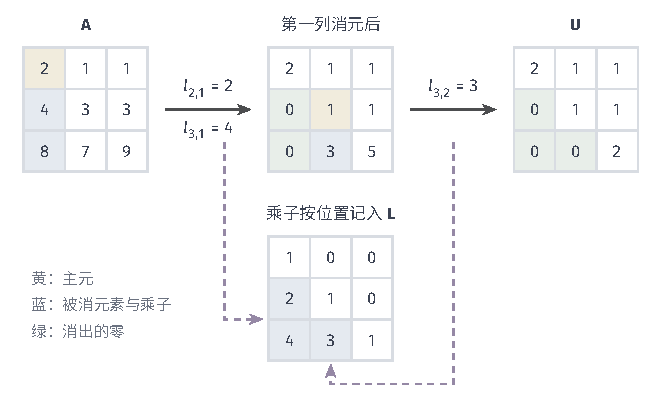
\includegraphics[width=112mm]{figures/00-shared/mathematical-preliminaries-upper/02-linear-spaces/tikz/comprehension-additions/linear-lu-elimination-steps.pdf}
  \caption{三阶矩阵的消元与LU因子。左起依次是$\bm A$、消去第一列后的矩阵与$\bm U$；
  黄色是当前主元，蓝色是待消去的元素，绿色是消出的零。箭头上的乘子等于被消元素除以主元，
  下方按原位置收集成单位下三角因子$\bm L$，满足$\bm L\bm U=\bm A$。}
  \label{fig:ls-lu-elimination-steps}
\end{figure}

\paragraph{求解$\bm L\bm y=\bm c$}
分解完成后处理右端。把$\bm b$按同一置换重排为$\bm c=\bm P\bm b$。由式~\eqref{eq:ls-palu}，原方程等价于$\bm L\bm U\bm x=\bm c$；令$\bm y=\bm U\bm x$，它分成$\bm L\bm y=\bm c$和$\bm U\bm x=\bm y$两个三角方程，依次求解。下三角方程的第一个方程只含$y_1$；解出后，第二个方程只剩$y_2$未知。如此从$i=1$到$d$逐个计算
\begin{equation}
 y_i=\frac{c_i-\sum_{j<i}l_{i,j}y_j}{l_{i,i}},
 \label{eq:ls-forward-substitution}
\end{equation}
右侧只用到已经算出的$y_1,\ldots,y_{i-1}$。这种求解顺序称为前代；只要对角元都不为零，它逐个唯一地给出解。本处$l_{i,i}=1$，除法可以省去。

\paragraph{求解$\bm U\bm x=\bm y$}
上三角方程的最后一个方程只含$x_d$，于是从$i=d$到$1$逐个计算
\begin{equation}
 x_i=\frac{y_i-\sum_{j>i}u_{i,j}x_j}{u_{i,i}},
 \label{eq:ls-back-substitution}
\end{equation}
右侧只用到已经算出的$x_{i+1},\ldots,x_d$。这种求解顺序称为回代，完成后得到的$\bm x$就是$\bm x_\star$。图~\ref{fig:ls-triangular-substitution-order}对比了两种顺序：前代自上而下，每个分量只依赖它上方已求出的分量；回代自下而上，依赖关系正好反过来。后面各节遇到三角方程时，直接调用前代和回代。

\begin{figure}[!htb]
  \centering
  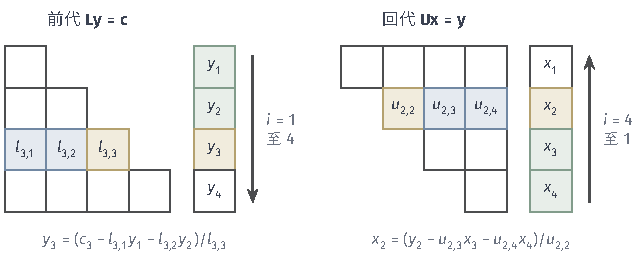
\includegraphics[width=109.1mm]{figures/01-basic-mathematics/03-vectors-matrices-and-multivariate-functions/tikz/c5-triangular-substitution-order/figure.pdf}
  \caption{前代与回代的计算顺序。左为四阶下三角方程，计算$y_3$时只用到第三行的蓝色元素与绿色的已算分量$y_1,y_2$；
  右为上三角方程，计算$x_2$时只用到$x_3,x_4$。黄色是当前用作除数的对角元与正在计算的分量，箭头是计算方向。}
  \label{fig:ls-triangular-substitution-order}
\end{figure}

\begin{example}[部分选主元LU的三步计算]
\label{ex:ls-lu-three-steps}
取
\[
 \bm A=\begin{bmatrix}1&3&4\\2&2&4\\1&2&5\end{bmatrix},\qquad
 \bm b=\begin{bmatrix}2\\4\\4\end{bmatrix}.
\]
第一步分解。第一列中绝对值最大的是第二行的$2$，交换第一、二行，$\bm P$随之交换。乘子$l_{2,1}=l_{3,1}=\tfrac12$，消元后两行变为$(0,2,2)$与$(0,1,3)$。第二列剩余元素中$|2|>|1|$，主元已在第二行，无需交换；乘子$l_{3,2}=\tfrac12$，第三行变为$(0,0,2)$。于是
\[
 \bm P=\begin{bmatrix}0&1&0\\1&0&0\\0&0&1\end{bmatrix},\
 \bm L=\begin{bmatrix}1&0&0\\\tfrac12&1&0\\\tfrac12&\tfrac12&1\end{bmatrix},\
 \bm U=\begin{bmatrix}2&2&4\\0&2&2\\0&0&2\end{bmatrix}.
\]
第二步前代。$\bm c=\bm P\bm b=(4,2,4)^\top$，依次得$y_1=4$，$y_2=2-\tfrac12\cdot4=0$，$y_3=4-\tfrac12\cdot4-\tfrac12\cdot0=2$。第三步回代：$x_3=2/2=1$，$x_2=(0-2\cdot1)/2=-1$，$x_1=(4-2\cdot(-1)-4\cdot1)/2=1$。所以$\bm x=(1,-1,1)^\top$，代回可验$\bm A\bm x=(2,4,4)^\top=\bm b$，也可直接验证$\bm L\bm U$等于交换前两行后的$\bm A$。
\end{example}

\subsubsection{算法分析}
\paragraph{正确性}
算法能否进行，取决于每一步是否有非零主元。部分选主元对任何非奇异矩阵都能进行；不选主元时则需要额外的条件，下面的定理给出这一条件，并说明分解在什么意义下唯一。

\begin{theorem}[LU分解的存在与唯一]
\label{thm:ls-lu-existence}
设$\bm A\in\mathbb R^{d\times d}$，记$\bm A_k$为其左上角$k$阶子矩阵。
\begin{enumerate}
 \item 若$\bm A$非奇异，则部分选主元消元的每一步都有非零主元，给出置换矩阵$\bm P$、元素满足$|l_{i,j}|\leq1$的单位下三角矩阵$\bm L$与非奇异上三角矩阵$\bm U$，使$\bm P\bm A=\bm L\bm U$。
 \item 不选主元时，$\bm A=\bm L\bm U$（$\bm L$单位下三角，$\bm U$非奇异上三角）存在，当且仅当$\det\bm A_k\neq0$对$k=1,\ldots,d$都成立；此时分解唯一。
\end{enumerate}
\end{theorem}
\begin{proof}
（1）第$k$步开始时$\bm W=\bm M\bm A$，其中$\bm M$是此前各次行交换与消元矩阵的乘积，可逆；$\bm W$的前$k-1$列已是对角元非零的上三角形状。若第$k$列从第$k$行起全为零，$\bm W$的前$k$列就都落在$\operatorname{span}\{\bm e_1,\ldots,\bm e_{k-1}\}$中而线性相关，$\bm A=\bm M^{-1}\bm W$随之奇异，矛盾。选出的主元绝对值最大，故$|l_{i,k}|\leq1$。消元过程可以倒过来读：$\bm U$的第$i$行等于$\bm P\bm A$的第$i$行减去$\bm U$前$i-1$行的$l_{i,k}$倍，移项就是$\bm L\bm U$的第$i$行，故$\bm P\bm A=\bm L\bm U$。

（2）若$\bm A=\bm L\bm U$，由三角形状，左上角$k$阶块满足$\bm A_k=\bm L_k\bm U_k$，故$\det\bm A_k=\prod_{i\leq k}u_{i,i}\neq0$。反之，设各$\det\bm A_k\neq0$，用归纳法说明不选主元时第$k$个主元非零：前$k-1$步只用了单位下三角的消元矩阵，$\bm W=\bm M\bm A$中$\bm M$单位下三角，于是$\bm W_k=\bm M_k\bm A_k$，$\det\bm W_k=\det\bm A_k\neq0$；而$\bm W_k$是上三角矩阵，前$k-1$个对角元非零，所以$w_{k,k}\neq0$。唯一性：若$\bm L_1\bm U_1=\bm L_2\bm U_2$，则$\bm L_2^{-1}\bm L_1=\bm U_2\bm U_1^{-1}$，左边单位下三角，右边上三角，只能都等于$\bm I_d$。
\end{proof}

定理的第一部分说明前代与回代给出的正是原方程的解：行交换只重排方程，不改变解。第二部分中的条件不能仅由$\bm A$非奇异推出，例如$\left[\begin{smallmatrix}0&1\\1&1\end{smallmatrix}\right]$可逆，第一个主元却为零。

\paragraph{数值敏感度}
部分选主元使$|l_{i,k}|\leq1$，但舍入的影响仍取决于消元中元素的增长，相应的误差界见第~\ref{sec:ls-numerical-stability}节。

\paragraph{计算代价}
第$k$步更新$(d-k)^2$个元素，一次稠密分解约需$\tfrac23d^3$次浮点运算；此后每个新右端只需一次前代和一次回代，约$2d^2$次运算。稀疏矩阵消元时，原来为零的位置会产生非零元，称为\term{填充}（fill-in），其多少取决于消元顺序，估计代价时须一并考虑。

\subsection{Cholesky分解}
\label{sec:ls-cholesky}

\subsubsection{主要思想}
设$\bm A\in\mathbb R^{d\times d}$实对称正定，$\bm b\in\mathbb R^d$，要求精确解$\bm x_\star$。核心思想是利用对称性，把LU中的两个三角因子取成互为转置的形式，即\term{Cholesky分解}（Cholesky decomposition）
\begin{equation}
 \bm A=\bm L\bm L^\top,
 \label{eq:matrix-analysis-cholesky}
\end{equation}
其中$\bm L$是对角元为正的下三角矩阵。这样只需构造一个因子$\bm L$，原方程$\bm L(\bm L^\top\bm x)=\bm b$就化为两个三角方程，用前代和回代各解一次。

\subsubsection{算法实现}
\paragraph{$\bm L\bm L^\top$分解}
将$\bm L$初始化为零矩阵，按$j=1,\ldots,d$逐列计算
\begin{equation}
\begin{gathered}
 l_{j,j}=\sqrt{a_{j,j}-\sum_{k<j}l_{j,k}^2},\\
 l_{i,j}=\frac{a_{i,j}-\sum_{k<j}l_{i,k}l_{j,k}}{l_{j,j}}\quad(i>j).
\end{gathered}
\label{eq:ls-cholesky-columns}
\end{equation}
这两式来自比较$\bm A$与$\bm L\bm L^\top$的元素：$\bm L\bm L^\top$的$(i,j)$元（$i\geq j$）是$\sum_{k\leq j}l_{i,k}l_{j,k}$，其中$k<j$的项只含已经完成的列，令它等于$a_{i,j}$，就能解出剩下的一项$l_{i,j}l_{j,j}$（$i=j$时是$l_{j,j}^2$）。因此每一列先算对角元，再算它下方的各元素，计算只读取$\bm A$的下三角部分。$\bm L^\top$不需要另作分解：它的$(i,j)$元就是$l_{j,i}$，由$\bm L$转置即得。

\paragraph{求解$\bm L\bm y=\bm b$}
用第~\ref{sec:ls-lu}节的前代~\eqref{eq:ls-forward-substitution}求解$\bm L\bm y=\bm b$，得到中间向量$\bm y$。与LU不同，这里$l_{i,i}$一般不等于$1$，前代公式中的除法要保留。

\paragraph{求解$\bm L^\top\bm x=\bm y$}
用回代~\eqref{eq:ls-back-substitution}求解$\bm L^\top\bm x=\bm y$，其中的上三角元素$(\bm L^\top)_{i,j}=l_{j,i}$直接从$\bm L$读出，完成后得到所求的$\bm x$。两次三角求解的次序来自$\bm L(\bm L^\top\bm x)=\bm b$：先解出括号内的$\bm y=\bm L^\top\bm x$，再由$\bm y$求$\bm x$。

\begin{example}[Cholesky分解的三步计算]
\label{ex:ls-cholesky-three-steps}
取
\[
 \bm A=\begin{bmatrix}4&2&2\\2&5&3\\2&3&6\end{bmatrix},\qquad
 \bm b=\begin{bmatrix}8\\10\\11\end{bmatrix}.
\]
逐列分解得$l_{1,1}=\sqrt4=2$，$l_{2,1}=l_{3,1}=2/2=1$；$l_{2,2}=\sqrt{5-1}=2$，$l_{3,2}=(3-1\cdot1)/2=1$；$l_{3,3}=\sqrt{6-1-1}=2$，即
\[
 \bm L=\begin{bmatrix}2&0&0\\1&2&0\\1&1&2\end{bmatrix}.
\]
前代解$\bm L\bm y=\bm b$：$y_1=8/2=4$，$y_2=(10-4)/2=3$，$y_3=(11-4-3)/2=2$。回代解$\bm L^\top\bm x=\bm y$：$x_3=2/2=1$，$x_2=(3-1)/2=1$，$x_1=(4-1-1)/2=1$。所以$\bm x=(1,1,1)^\top$，代回可验$\bm A\bm x=\bm b$。
\end{example}

\subsubsection{算法分析}
\paragraph{正确性}
逐列构造能否进行，取决于每次开方的数是否为正。下面的定理说明，这恰好由正定性保证，而且正定性也是分解存在的必要条件。

\begin{theorem}[Cholesky分解的存在与唯一]
\label{thm:ls-cholesky-existence}
设$\bm A\in\mathbb R^{d\times d}$对称。存在对角元为正的下三角矩阵$\bm L$使$\bm A=\bm L\bm L^\top$，当且仅当$\bm A\succ0$；此时$\bm L$唯一，并由式~\eqref{eq:ls-cholesky-columns}给出。
\end{theorem}
\begin{proof}
必要性：$\bm L$的对角元为正，故可逆；对非零$\bm v$有$\bm v^\top\bm A\bm v=\lVert\bm L^\top\bm v\rVert_2^2>0$。充分性对阶数归纳。把$\bm A$按首行首列分块为$\left[\begin{smallmatrix}a_{1,1}&\bm a^\top\\\bm a&\bm A_{22}\end{smallmatrix}\right]$，正定性给出$a_{1,1}=\bm e_1^\top\bm A\bm e_1>0$，所以$l_{1,1}=\sqrt{a_{1,1}}$有定义，第一列其余元素为$\bm a/l_{1,1}$。对$\bm v=(v_1,\bm w^\top)^\top$关于首变量配方，
\[
\begin{aligned}
 \bm v^\top\bm A\bm v
 &=a_{1,1}\Bigl(v_1+\frac{\bm a^\top\bm w}{a_{1,1}}\Bigr)^2\\
 &\quad+\bm w^\top\Bigl(\bm A_{22}-\frac{\bm a\bm a^\top}{a_{1,1}}\Bigr)\bm w .
\end{aligned}
\]
对任意非零$\bm w$取$v_1=-\bm a^\top\bm w/a_{1,1}$，左边为正，故剩余矩阵$\bm A_{22}-\bm a\bm a^\top/a_{1,1}$仍正定；后面各列的计算正是对它重复同样的步骤，由归纳假设每一步开方的数都为正。唯一性：对角元取正后，式~\eqref{eq:ls-cholesky-columns}逐个唯一地确定每个元素。
\end{proof}

由$\bm A=\bm L\bm L^\top$，算出的$\bm x$满足$\bm A\bm x=\bm L(\bm L^\top\bm x)=\bm L\bm y=\bm b$。

\paragraph{数值敏感度}
$a_{j,j}=\sum_{k\leq j}l_{j,k}^2$给出$|l_{j,k}|\leq\sqrt{a_{j,j}}$，因子的元素不会增长，因此分解不选主元也是后向稳定的（第~\ref{sec:ls-numerical-stability}节）；解的误差仍由$\bm A$的条件数决定（第~\ref{sec:ls-matrix-condition-number}节）。

\paragraph{计算代价}
稠密分解约需$\tfrac13d^3$次运算，是LU的一半，存储也只需一个三角因子。

\subsection{分块LDL分解}
\label{sec:ls-ldlt}

\subsubsection{主要思想}
设$\bm A\in\mathbb R^{d\times d}$实对称非奇异，但不一定正定，$\bm b\in\mathbb R^d$，要求唯一精确解$\bm x_\star$。这时Cholesky分解的根号内可能出现负数。分块LDL分解不开方，而把主元连同它的正负号保留在块对角矩阵$\bm D$中，构造
\begin{equation}
 \bm P\bm A\bm P^\top=\bm L\bm D\bm L^\top,
 \label{eq:ls-ldlt}
\end{equation}
其中$\bm P$是置换矩阵，$\bm L$是单位下三角矩阵，$\bm D$由可逆的一阶和二阶对称块组成。对称置换同时交换行与列，矩阵保持对称；允许二阶块，是因为对角元可能全为零，这时找不到一阶主元。

\subsubsection{算法实现}
超参数是选块策略。为使给定数据下的计算可以复算，这里采用一个默认的代数规则：当前剩余矩阵有非零对角元时，取绝对值最大的对角元作一阶块；对角元全为零时，取绝对值最大的非零非对角元及其两个下标组成二阶块，绝对值相同时按下标顺序选择。后一种块形如$\left[\begin{smallmatrix}0&a\\a&0\end{smallmatrix}\right]$，$a\neq0$，行列式$-a^2\neq0$，所以可逆。这一规则只保证构造能够进行，并不保证数值稳定。

\paragraph{选块与对称交换}
初始化$\bm W=\bm A$、$\bm L=\bm I_d$、$\bm P=\bm I_d$，$\bm D$为空。每一轮先按选块策略把主元下标交换到剩余矩阵的前端：同时交换$\bm W$的相应行与列，对$\bm P$作同样的行交换，$\bm L$中已经算出的乘子也交换相应两行。交换后把当前剩余矩阵写成
\[
 \begin{bmatrix}\bm E&\bm C^\top\\\bm C&\bm F\end{bmatrix},
\]
其中$\bm E$是选出的一阶或二阶可逆块。

\paragraph{块消元}
乘子块$\bm M$满足$\bm M\bm E=\bm C$，逐行求解这个一阶或二阶方程即得。把$\bm M$写入$\bm L$中主元块下方的位置，把$\bm E$放入$\bm D$的下一个对角块，再把剩余矩阵更新为
\[
 \bm F-\bm M\bm C^\top .
\]
它仍是对称矩阵，只需计算下三角部分。对这个更小的矩阵重复选块与消元，直到剩余矩阵为空。

\paragraph{三段求解}
由式~\eqref{eq:ls-ldlt}，$\bm A\bm x=\bm b$等价于$\bm L\bm D\bm L^\top(\bm P\bm x)=\bm P\bm b$。先把右端重排为$\bm c=\bm P\bm b$，用前代求解$\bm L\bm y=\bm c$。接着按$\bm D$的对角块逐个求解$\bm D\bm z=\bm y$：一阶块直接作标量除法；对二阶块$\left[\begin{smallmatrix}e_{1,1}&e_{1,2}\\e_{1,2}&e_{2,2}\end{smallmatrix}\right]$，把它对应的两个分量记为$(y_1,y_2)$与$(z_1,z_2)$，由二阶逆矩阵公式得
\[
\begin{gathered}
 z_1=\frac{e_{2,2}y_1-e_{1,2}y_2}{e_{1,1}e_{2,2}-e_{1,2}^2},\\
 z_2=\frac{e_{1,1}y_2-e_{1,2}y_1}{e_{1,1}e_{2,2}-e_{1,2}^2},
\end{gathered}
\]
分母因所选块可逆而非零。最后用回代求解$\bm L^\top\bm w=\bm z$，此时$\bm w=\bm P\bm x$，再按$\bm x=\bm P^\top\bm w$恢复未知量的原次序，得到所求的$\bm x$。

\begin{example}[需要二阶块的LDL分解]
\label{ex:ls-ldlt-two-by-two}
取
\[
 \bm A=\begin{bmatrix}0&2&1\\2&0&1\\1&1&0\end{bmatrix},\qquad
 \bm b=\begin{bmatrix}3\\3\\2\end{bmatrix}.
\]
对角元全为零，绝对值最大的非对角元是$a_{1,2}=2$，它的两个下标已在前端，$\bm P=\bm I_3$，$\bm E=\left[\begin{smallmatrix}0&2\\2&0\end{smallmatrix}\right]$，$\bm C=(1,1)$，$\bm F=0$。由$\bm M\bm E=\bm C$得$\bm M=(\tfrac12,\tfrac12)$，剩余矩阵为$0-\bm M\bm C^\top=-1$，于是$\bm D=\operatorname{diag}(\bm E,-1)$，$\bm L$的第三行为$(\tfrac12,\tfrac12,1)$。求解时，前代得$\bm y=(3,3,2-\tfrac32-\tfrac32)^\top=(3,3,-1)^\top$；二阶块给出$z_1=z_2=(0-6)/(-4)=\tfrac32$，一阶块给出$z_3=1$；回代得$w_3=1$，$w_2=w_1=\tfrac32-\tfrac12=1$。因此$\bm x=(1,1,1)^\top$，代回可验$\bm A\bm x=\bm b$。
\end{example}

\subsubsection{算法分析}
\paragraph{正确性}
一步块消元可以写成
\[
\begin{aligned}
 \begin{bmatrix}\bm E&\bm C^\top\\\bm C&\bm F\end{bmatrix}
 &=\begin{bmatrix}\bm I&\bm0\\\bm M&\bm I\end{bmatrix}
 \begin{bmatrix}\bm E&\bm0\\\bm0&\bm F-\bm M\bm C^\top\end{bmatrix}\\
 &\quad\cdot\begin{bmatrix}\bm I&\bm M^\top\\\bm0&\bm I\end{bmatrix},
\end{aligned}
\]
乘开并利用$\bm M\bm E=\bm C$、$\bm E^\top=\bm E$即可验证。两侧单位块三角因子的行列式为$1$，对称置换也不改变行列式，所以每一轮的剩余矩阵都与$\bm A$一样非奇异；非奇异的对称矩阵不是零矩阵，选块规则总能选出可逆块。逐轮累积对称置换与乘子即得式~\eqref{eq:ls-ldlt}，前代、块对角求解、回代与还原次序因而给出原方程的解。$\bm D$中的负主元或不定二阶块只说明$\bm A$有使二次型为负的方向，并不妨碍可逆求解。

\paragraph{数值敏感度}
存在可逆主元并不等于稳定：主元块相对很小时乘子很大，剩余矩阵的元素随之增长。实用的选块策略要控制这种增长，Bunch--Kaufman策略就是一例，它按当前对角元与所在列最大非对角元的相对大小，决定取一阶块还是二阶块。

\paragraph{计算代价}
稠密计算约需$\tfrac13d^3$次运算，存储约$\tfrac12d^2$个元素，利用对称性比直接用LU减少一半。

\subsection{分块消元}
\label{sec:ls-block-elimination}

\subsubsection{主要思想}
设非奇异矩阵$\bm A$、右端$\bm b$与待求的$\bm x$按两组未知量分块为
\[
 \bm A=\begin{bmatrix}\bm B&\bm C\\\bm D&\bm E\end{bmatrix},\quad
 \bm b=\begin{bmatrix}\bm f\\\bm g\end{bmatrix},\quad
 \bm x=\begin{bmatrix}\bm u\\\bm v\end{bmatrix},
\]
其中$\bm B\in\mathbb R^{p\times p}$可逆，$\bm E\in\mathbb R^{q\times q}$，$p+q=d$。分块只是输入$\bm A,\bm b$的一种写法，求解目标仍是精确解。做法是先用第一组方程把$\bm u$用$\bm v$表示，代入第二组方程消去$\bm u$，求解只含$\bm v$的较小方程，再回头恢复$\bm u$。

\subsubsection{算法实现}
\paragraph{用$\bm B$的因子求解}
按$\bm B$的结构调用前面的LU分解、Cholesky分解或分块LDL分解，得到$\bm B$的因子；已有分解时直接复用。然后用这组因子求解$\bm B\bm Z=\bm C$的各列和$\bm B\bm z=\bm f$，得到$\bm Z\in\mathbb R^{p\times q}$与$\bm z\in\mathbb R^p$。它们分别是$\bm B^{-1}\bm C$与$\bm B^{-1}\bm f$，但计算时只做前代与回代，不形成$\bm B^{-1}$。

\paragraph{形成Schur补方程}
第一组方程$\bm B\bm u+\bm C\bm v=\bm f$给出$\bm u=\bm z-\bm Z\bm v$。代入第二组方程$\bm D\bm u+\bm E\bm v=\bm g$，得到约化方程
\begin{equation}
 \bm S\bm v=\bm h,\qquad
 \bm S=\bm E-\bm D\bm Z,\quad
 \bm h=\bm g-\bm D\bm z .
 \label{eq:ls-schur-reduced-system}
\end{equation}
$q$阶矩阵$\bm S=\bm E-\bm D\bm B^{-1}\bm C$称为$\bm A$关于被消块$\bm B$的\term{Schur补}（Schur complement）。消去$\bm u$时，系数和右端都要扣除经由$\bm u$传来的部分，所以$\bm S$与$\bm h$必须同时形成。图~\ref{fig:ls-block-elimination-schur}把这一步画成增广分块矩阵的块行变换：左下块被消成零，右下块和右端分别换成$\bm S$与$\bm h$，剩下的是块上三角方程。

\begin{figure}[!htb]
  \centering
  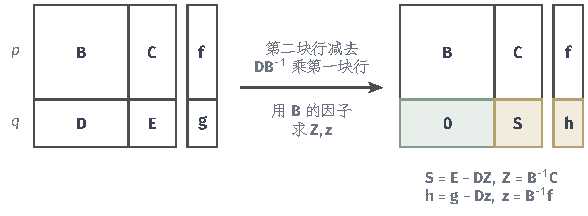
\includegraphics[width=99.547mm]{figures/01-basic-mathematics/03-vectors-matrices-and-multivariate-functions/tikz/c5-block-elimination-schur/figure.pdf}
  \caption{分块消元的结构。左为增广分块矩阵$[\bm A\mid\bm b]$，两组未知量的个数分别为$p$与$q$；
  第二块行减去$\bm D\bm B^{-1}$乘第一块行后，左下块变为零（绿色），右下块与右端变为Schur补$\bm S$及$\bm h$（黄色）。
  $\bm Z,\bm z$由$\bm B$的因子求得，不形成$\bm B^{-1}$。}
  \label{fig:ls-block-elimination-schur}
\end{figure}

\paragraph{求解$\bm S\bm v=\bm h$并恢复$\bm u$}
按$\bm S$的结构调用已有的直接法解出$\bm v$。$\bm A$与$\bm B$都非奇异时$\bm S$也非奇异（见定理~\ref{thm:ls-schur-complement}），这一步给出唯一结果。最后计算$\bm u=\bm z-\bm Z\bm v$，按原分组拼成$\bm x=(\bm u^\top,\bm v^\top)^\top$，完成原方程的求解。

\begin{example}[二阶贯穿例的分块消元]
\label{ex:ls-block-elimination-run}
取$\bm A=\left[\begin{smallmatrix}4&1\\1&3\end{smallmatrix}\right]$，$\bm b=(1,2)^\top$，令$p=q=1$，即$\bm B=4$，$\bm C=\bm D=1$，$\bm E=3$，$\bm f=1$，$\bm g=2$。第一步得$\bm Z=\tfrac14$，$\bm z=\tfrac14$。第二步形成$\bm S=3-\tfrac14=\tfrac{11}4$，$\bm h=2-\tfrac14=\tfrac74$。第三步解出$v=\tfrac74\big/\tfrac{11}4=\tfrac7{11}$，再得$u=\tfrac14-\tfrac14\cdot\tfrac7{11}=\tfrac1{11}$。代回可验$4\cdot\tfrac1{11}+\tfrac7{11}=1$，$\tfrac1{11}+3\cdot\tfrac7{11}=2$；又$\det\bm A=4\cdot\tfrac{11}4=11$，与下面定理中的行列式公式一致。
\end{example}

\subsubsection{算法分析}
\paragraph{正确性}
按构造，$(\bm u,\bm v)$满足第一组方程，而在$\bm u=\bm z-\bm Z\bm v$下第二组方程恰好等价于$\bm S\bm v=\bm h$，所以算法给出原方程的解。把消元写成矩阵乘法，还能读出整体可逆性、逆矩阵和正定性。

\begin{theorem}[Schur补的行列式、逆与正定性]
\label{thm:ls-schur-complement}
设$\bm B$可逆，$\bm S=\bm E-\bm D\bm B^{-1}\bm C$。则$\det\bm A=\det\bm B\det\bm S$，$\bm A$可逆当且仅当$\bm S$可逆，此时
\begin{equation}
 \bm A^{-1}=
 \begin{bmatrix}
  \bm B^{-1}+\bm B^{-1}\bm C\bm S^{-1}\bm D\bm B^{-1}
  &-\bm B^{-1}\bm C\bm S^{-1}\\
  -\bm S^{-1}\bm D\bm B^{-1}&\bm S^{-1}
 \end{bmatrix}.
 \label{eq:matrix-analysis-block-inverse}
\end{equation}
同理，若$\bm E$可逆，则$\det\bm A=\det\bm E\det(\bm B-\bm C\bm E^{-1}\bm D)$。若$\bm A$对称（$\bm D=\bm C^\top$）且$\bm B\succ0$，则
\begin{equation}
 \bm A\succ0\quad\Longleftrightarrow\quad
 \bm E-\bm C^\top\bm B^{-1}\bm C\succ0.
 \label{eq:matrix-analysis-schur-positive-definite}
\end{equation}
\end{theorem}
\begin{proof}
消去左下块再消去右上块，得到
\[
 \bm A=
 \begin{bmatrix}\bm I&\bm0\\\bm D\bm B^{-1}&\bm I\end{bmatrix}
 \begin{bmatrix}\bm B&\bm0\\\bm0&\bm S\end{bmatrix}
 \begin{bmatrix}\bm I&\bm B^{-1}\bm C\\\bm0&\bm I\end{bmatrix},
\]
按分块乘法相乘即可验证。两侧单位块三角因子的行列式为$1$，取行列式得$\det\bm A=\det\bm B\det\bm S$，又$\det\bm B\neq0$，故$\bm A$可逆当且仅当$\bm S$可逆。此时三个因子分别求逆：单位块三角因子的逆只需把非对角块变号，中间因子的逆是$\operatorname{diag}(\bm B^{-1},\bm S^{-1})$，按相反顺序相乘即得式~\eqref{eq:matrix-analysis-block-inverse}。$\bm E$可逆时先消去$\bm v$，同样的论证给出第二个行列式公式。对称时右侧因子是左侧因子的转置，上式写成$\bm A=\bm G\operatorname{diag}(\bm B,\bm S)\bm G^\top$，其中$\bm G$可逆；展开二次型即是对$\bm u$配方：
\[
 \bm x^\top\bm A\bm x
 =(\bm u+\bm B^{-1}\bm C\bm v)^\top\bm B(\bm u+\bm B^{-1}\bm C\bm v)+\bm v^\top\bm S\bm v .
\]
$\bm G^\top$可逆，所以$\bm A\succ0$当且仅当$\operatorname{diag}(\bm B,\bm S)\succ0$；已知$\bm B\succ0$，这又等价于$\bm S\succ0$。
\end{proof}

\paragraph{数值敏感度}
误差来自三处：用$\bm B$的因子求$\bm Z$与$\bm z$，形成$\bm S=\bm E-\bm D\bm Z$时的相减，以及约化方程的求解。$\bm B$病态时，$\bm Z$与$\bm z$的误差会传入$\bm S$与$\bm h$，相当于块层面的小主元，这时应换一种分组。

\paragraph{计算代价}
若$\bm B$稠密，各步合计与对整个$\bm A$作LU同为$(p+q)^3$量级，单纯改写成分块形式并不省事；节省须依赖被消块易于求解（例如块对角，各小块可以分别分解）或保留块较小。

\subsection{低秩更新下的求解}
\label{sec:ls-woodbury}

\subsubsection{主要思想}
设新的系数矩阵具有已知结构
\[
 \bm A=\bm A_0+\bm U\bm C\bm V^\top,
\]
其中$\bm A_0\in\mathbb R^{d\times d}$非奇异，$\bm U,\bm V\in\mathbb R^{d\times k}$，$\bm C\in\mathbb R^{k\times k}$，$k\ll d$，且$\bm A$非奇异；要求$\bm A\bm x=\bm b$的精确解。更新表示是输入矩阵的结构信息，$\bm A_0$已有的分解只在内部复用。核心做法是把修改项的作用集中到$k$维辅助量$\bm C\bm V^\top\bm x$上：用旧矩阵求解若干次，再解一个$k$阶小方程，从而避免重新分解$d$阶矩阵。

\subsubsection{算法实现}
\paragraph{用旧因子求解}
先取得$\bm A_0$的分解。它通常已经存在，可以直接复用；尚无分解时先按$\bm A_0$的结构调用前面的方法求得。下面关于节省计算的比较，以分解已经存在为前提。用这组因子求解$\bm A_0\bm u=\bm b$，得到未作更新时的解$\bm u$；再对$\bm U$的$k$列复用同一组因子，求解$\bm A_0\bm Z=\bm U$，得到$\bm Z\in\mathbb R^{d\times k}$，它记录修改方向经$\bm A_0^{-1}$作用后的结果。

\paragraph{形成小系统}
形成$k$阶矩阵与$k$维向量
\[
 \bm K=\bm I_k+\bm C\bm V^\top\bm Z,\qquad
 \bm h=\bm C\bm V^\top\bm u .
\]
计算时先算$\bm V^\top\bm Z$与$\bm V^\top\bm u$，再左乘$\bm C$，全程不形成新的$d$阶矩阵。

\paragraph{求解小系统并修正}
调用已有的直接法求解$\bm K\bm z=\bm h$，再计算$\bm x=\bm u-\bm Z\bm z$，得到新方程的解。

\begin{example}[秩一更新的计算]
\label{ex:ls-woodbury-rank-one}
二阶贯穿例$\bm A=\left[\begin{smallmatrix}4&1\\1&3\end{smallmatrix}\right]$可以写成$\bm A_0=\operatorname{diag}(3,2)$加上秩一修改，$\bm U=\bm V=(1,1)^\top$，$\bm C=1$；右端$\bm b=(1,2)^\top$。对角的$\bm A_0$求解只需逐个相除：$\bm u=(\tfrac13,1)^\top$，$\bm Z=(\tfrac13,\tfrac12)^\top$。小系统是标量：$\bm K=1+\tfrac13+\tfrac12=\tfrac{11}6$，$\bm h=\tfrac13+1=\tfrac43$，于是$\bm z=\tfrac43\cdot\tfrac6{11}=\tfrac8{11}$。修正后
\[
 \bm x=\begin{bmatrix}\tfrac13\\1\end{bmatrix}-\frac8{11}\begin{bmatrix}\tfrac13\\\tfrac12\end{bmatrix}
 =\begin{bmatrix}\tfrac1{11}\\\tfrac7{11}\end{bmatrix},
\]
与例~\ref{ex:ls-block-elimination-run}的结果一致，全程没有分解$\bm A$本身。
\end{example}

\subsubsection{算法分析}
\paragraph{正确性}
令$\bm z=\bm C\bm V^\top\bm x$，原方程写成$\bm A_0\bm x+\bm U\bm z=\bm b$，等价于$\bm x=\bm u-\bm Z\bm z$；代回$\bm z$的定义得$\bm z=\bm h-\bm C\bm V^\top\bm Z\bm z$，即$\bm K\bm z=\bm h$。反过来，若$\bm K\bm z=\bm h$且$\bm x=\bm u-\bm Z\bm z$，则$\bm C\bm V^\top\bm x=\bm h-(\bm K-\bm I_k)\bm z=\bm z$，从而$\bm A\bm x=\bm A_0\bm x+\bm U\bm z=\bm b$。所以小系统与原方程等价。把这一等价关系对任意右端写成矩阵形式，就得到下面的可逆性判据与逆矩阵公式。

\begin{theorem}[Woodbury恒等式]
\label{thm:ls-woodbury}
设$\bm A_0\in\mathbb R^{d\times d}$可逆，$\bm U,\bm V\in\mathbb R^{d\times k}$，$\bm C\in\mathbb R^{k\times k}$，记$\bm K=\bm I_k+\bm C\bm V^\top\bm A_0^{-1}\bm U$。则
\[
 \det(\bm A_0+\bm U\bm C\bm V^\top)=\det\bm A_0\det\bm K,
\]
因而$\bm A_0+\bm U\bm C\bm V^\top$可逆当且仅当$\bm K$可逆。若$\bm C$也可逆且$\bm K$可逆，则成立\term{Woodbury恒等式}（Woodbury identity）
\begin{equation}
\begin{aligned}
 &(\bm A_0+\bm U\bm C\bm V^\top)^{-1}\\
 &=\bm A_0^{-1}-\bm A_0^{-1}\bm U
 (\bm C^{-1}+\bm V^\top\bm A_0^{-1}\bm U)^{-1}
 \bm V^\top\bm A_0^{-1}.
\end{aligned}
\label{eq:matrix-analysis-woodbury}
\end{equation}
\end{theorem}
\begin{proof}
记$\bm Z=\bm A_0^{-1}\bm U$，则$\bm A_0+\bm U\bm C\bm V^\top=\bm A_0(\bm I_d+\bm Z\bm C\bm V^\top)$。对分块矩阵$\left[\begin{smallmatrix}\bm I_d&-\bm Z\\\bm C\bm V^\top&\bm I_k\end{smallmatrix}\right]$分别消去两个单位对角块，由定理~\ref{thm:ls-schur-complement}的两个行列式公式得$\det(\bm I_d+\bm Z\bm C\bm V^\top)=\det(\bm I_k+\bm C\bm V^\top\bm Z)=\det\bm K$，第一个结论成立。$\bm C$可逆时$\bm K=\bm C(\bm C^{-1}+\bm V^\top\bm A_0^{-1}\bm U)$，括号内的矩阵随$\bm K$可逆。由上面的等价关系，对任意$\bm b$，新方程的解为$\bm x=\bm u-\bm Z\bm K^{-1}\bm C\bm V^\top\bm u$，其中$\bm u=\bm A_0^{-1}\bm b$；代入$\bm K^{-1}\bm C=(\bm C^{-1}+\bm V^\top\bm A_0^{-1}\bm U)^{-1}$，并因$\bm b$任意而去掉右端，即得式~\eqref{eq:matrix-analysis-woodbury}。
\end{proof}

判据部分允许$\bm C$奇异，这正是算法只使用$\bm K$、不使用$\bm C^{-1}$的原因。秩一修改最常见，此时定理化为一个只含标量分母的公式。

\begin{theorem}[Sherman--Morrison公式]
\label{thm:ls-sherman-morrison}
设$\bm A_0\in\mathbb R^{d\times d}$可逆，$\bm p,\bm q\in\mathbb R^d$。则$\bm A_0+\bm p\bm q^\top$可逆当且仅当$1+\bm q^\top\bm A_0^{-1}\bm p\neq0$，此时
\[
 (\bm A_0+\bm p\bm q^\top)^{-1}
 =\bm A_0^{-1}-\frac{\bm A_0^{-1}\bm p\bm q^\top\bm A_0^{-1}}{1+\bm q^\top\bm A_0^{-1}\bm p}.
\]
\end{theorem}
\begin{proof}
在定理~\ref{thm:ls-woodbury}中取$k=1$、$\bm U=\bm p$、$\bm V=\bm q$、$\bm C=1$，则$\bm K=1+\bm q^\top\bm A_0^{-1}\bm p$是标量，$(\bm C^{-1}+\bm V^\top\bm A_0^{-1}\bm U)^{-1}=1/\bm K$，代入式~\eqref{eq:matrix-analysis-woodbury}即得。
\end{proof}

\paragraph{数值敏感度}
代数恒等式并不自动保证数值稳定。$\bm K$接近奇异时，小系统的求解会放大误差；$\bm A_0$的求解本身敏感时，$\bm u$与$\bm Z$的误差即使在$\bm A$良态时也会进入结果；$\bm u$与$\bm Z\bm z$大小相近时，相减还会发生相消。

\paragraph{计算代价}
已有因子时，$k+1$个右端的三角求解约需$O(kd^2)$次运算，形成$\bm V^\top\bm Z$约需$O(k^2d)$，求解小系统约需$O(k^3)$，合计$O(kd^2+k^2d+k^3)$；优势来自$k$远小于$d$，此时远少于重新分解的$\tfrac23d^3$。
